
%% bare_conf.tex
%% V1.4b
%% 2015/08/26
%% by Michael Shell
%% See:
%% http://www.michaelshell.org/
%% for current contact information.
%%
%% This is a skeleton file demonstrating the use of IEEEtran.cls
%% (requires IEEEtran.cls version 1.8b or later) with an IEEE
%% conference paper.
%%
%% Support sites:
%% http://www.michaelshell.org/tex/ieeetran/
%% http://www.ctan.org/pkg/ieeetran
%% and
%% http://www.ieee.org/

%%*************************************************************************
%% Legal Notice:
%% This code is offered as-is without any warranty either expressed or
%% implied; without even the implied warranty of MERCHANTABILITY or
%% FITNESS FOR A PARTICULAR PURPOSE!
%% User assumes all risk.
%% In no event shall the IEEE or any contributor to this code be liable for
%% any damages or losses, including, but not limited to, incidental,
%% consequential, or any other damages, resulting from the use or misuse
%% of any information contained here.
%%
%% All comments are the opinions of their respective authors and are not
%% necessarily endorsed by the IEEE.
%%
%% This work is distributed under the LaTeX Project Public License (LPPL)
%% ( http://www.latex-project.org/ ) version 1.3, and may be freely used,
%% distributed and modified. A copy of the LPPL, version 1.3, is included
%% in the base LaTeX documentation of all distributions of LaTeX released
%% 2003/12/01 or later.
%% Retain all contribution notices and credits.
%% ** Modified files should be clearly indicated as such, including  **
%% ** renaming them and changing author support contact information. **
%%*************************************************************************


% *** Authors should verify (and, if needed, correct) their LaTeX system  ***
% *** with the testflow diagnostic prior to trusting their LaTeX platform ***
% *** with production work. The IEEE's font choices and paper sizes can   ***
% *** trigger bugs that do not appear when using other class files.       ***                          ***
% The testflow support page is at:
% http://www.michaelshell.org/tex/testflow/



\documentclass[conference]{IEEEtran}
% Some Computer Society conferences also require the compsoc mode option,
% but others use the standard conference format.
%
% If IEEEtran.cls has not been installed into the LaTeX system files,
% manually specify the path to it like:
% \documentclass[conference]{../sty/IEEEtran}





% Some very useful LaTeX packages include:
% (uncomment the ones you want to load)


% *** MISC UTILITY PACKAGES ***
%
%\usepackage{ifpdf}
% Heiko Oberdiek's ifpdf.sty is very useful if you need conditional
% compilation based on whether the output is pdf or dvi.
% usage:
% \ifpdf
%   % pdf code
% \else
%   % dvi code
% \fi
% The latest version of ifpdf.sty can be obtained from:
% http://www.ctan.org/pkg/ifpdf
% Also, note that IEEEtran.cls V1.7 and later provides a builtin
% \ifCLASSINFOpdf conditional that works the same way.
% When switching from latex to pdflatex and vice-versa, the compiler may
% have to be run twice to clear warning/error messages.






% *** CITATION PACKAGES ***
%
%\usepackage{cite}
% cite.sty was written by Donald Arseneau
% V1.6 and later of IEEEtran pre-defines the format of the cite.sty package
% \cite{} output to follow that of the IEEE. Loading the cite package will
% result in citation numbers being automatically sorted and properly
% "compressed/ranged". e.g., [1], [9], [2], [7], [5], [6] without using
% cite.sty will become [1], [2], [5]--[7], [9] using cite.sty. cite.sty's
% \cite will automatically add leading space, if needed. Use cite.sty's
% noadjust option (cite.sty V3.8 and later) if you want to turn this off
% such as if a citation ever needs to be enclosed in parenthesis.
% cite.sty is already installed on most LaTeX systems. Be sure and use
% version 5.0 (2009-03-20) and later if using hyperref.sty.
% The latest version can be obtained at:
% http://www.ctan.org/pkg/cite
% The documentation is contained in the cite.sty file itself.






% *** GRAPHICS RELATED PACKAGES ***
%
\ifCLASSINFOpdf
  % \usepackage[pdftex]{graphicx}
  % declare the path(s) where your graphic files are
  % \graphicspath{{../pdf/}{../jpeg/}}
  % and their extensions so you won't have to specify these with
  % every instance of \includegraphics
  % \DeclareGraphicsExtensions{.pdf,.jpeg,.png}
\else
  % or other class option (dvipsone, dvipdf, if not using dvips). graphicx
  % will default to the driver specified in the system graphics.cfg if no
  % driver is specified.
  % \usepackage[dvips]{graphicx}
  % declare the path(s) where your graphic files are
  % \graphicspath{{../eps/}}
  % and their extensions so you won't have to specify these with
  % every instance of \includegraphics
  % \DeclareGraphicsExtensions{.eps}
\fi
% graphicx was written by David Carlisle and Sebastian Rahtz. It is
% required if you want graphics, photos, etc. graphicx.sty is already
% installed on most LaTeX systems. The latest version and documentation
% can be obtained at:
% http://www.ctan.org/pkg/graphicx
% Another good source of documentation is "Using Imported Graphics in
% LaTeX2e" by Keith Reckdahl which can be found at:
% http://www.ctan.org/pkg/epslatex
%
% latex, and pdflatex in dvi mode, support graphics in encapsulated
% postscript (.eps) format. pdflatex in pdf mode supports graphics
% in .pdf, .jpeg, .png and .mps (metapost) formats. Users should ensure
% that all non-photo figures use a vector format (.eps, .pdf, .mps) and
% not a bitmapped formats (.jpeg, .png). The IEEE frowns on bitmapped formats
% which can result in "jaggedy"/blurry rendering of lines and letters as
% well as large increases in file sizes.
%
% You can find documentation about the pdfTeX application at:
% http://www.tug.org/applications/pdftex





% *** MATH PACKAGES ***
%
%\usepackage{amsmath}
% A popular package from the American Mathematical Society that provides
% many useful and powerful commands for dealing with mathematics.
%
% Note that the amsmath package sets \interdisplaylinepenalty to 10000
% thus preventing page breaks from occurring within multiline equations. Use:
%\interdisplaylinepenalty=2500
% after loading amsmath to restore such page breaks as IEEEtran.cls normally
% does. amsmath.sty is already installed on most LaTeX systems. The latest
% version and documentation can be obtained at:
% http://www.ctan.org/pkg/amsmath





% *** SPECIALIZED LIST PACKAGES ***
%
%\usepackage{algorithmic}
% algorithmic.sty was written by Peter Williams and Rogerio Brito.
% This package provides an algorithmic environment fo describing algorithms.
% You can use the algorithmic environment in-text or within a figure
% environment to provide for a floating algorithm. Do NOT use the algorithm
% floating environment provided by algorithm.sty (by the same authors) or
% algorithm2e.sty (by Christophe Fiorio) as the IEEE does not use dedicated
% algorithm float types and packages that provide these will not provide
% correct IEEE style captions. The latest version and documentation of
% algorithmic.sty can be obtained at:
% http://www.ctan.org/pkg/algorithms
% Also of interest may be the (relatively newer and more customizable)
% algorithmicx.sty package by Szasz Janos:
% http://www.ctan.org/pkg/algorithmicx




% *** ALIGNMENT PACKAGES ***
%
%\usepackage{array}
% Frank Mittelbach's and David Carlisle's array.sty patches and improves
% the standard LaTeX2e array and tabular environments to provide better
% appearance and additional user controls. As the default LaTeX2e table
% generation code is lacking to the point of almost being broken with
% respect to the quality of the end results, all users are strongly
% advised to use an enhanced (at the very least that provided by array.sty)
% set of table tools. array.sty is already installed on most systems. The
% latest version and documentation can be obtained at:
% http://www.ctan.org/pkg/array


% IEEEtran contains the IEEEeqnarray family of commands that can be used to
% generate multiline equations as well as matrices, tables, etc., of high
% quality.




% *** SUBFIGURE PACKAGES ***
%\ifCLASSOPTIONcompsoc
%  \usepackage[caption=false,font=normalsize,labelfont=sf,textfont=sf]{subfig}
%\else
%  \usepackage[caption=false,font=footnotesize]{subfig}
%\fi
% subfiguresty, written by Steven Douglas Cochran, is the modern replacement
% for subfigure.sty, the latter of which is no longer maintained and is
% incompatible with some LaTeX packages including fixltx2e. However,
% subfiguresty requires and automatically loads Axel Sommerfeldt's caption.sty
% which will override IEEEtran.cls' handling of captions and this will result
% in non-IEEE style figure/table captions. To prevent this problem, be sure
% and invoke subfiguresty's "caption=false" package option (available since
% subfiguresty version 1.3, 2005/06/28) as this is will preserve IEEEtran.cls
% handling of captions.
% Note that the Computer Society format requires a larger sans serif font
% than the serif footnote size font used in traditional IEEE formatting
% and thus the need to invoke different subfiguresty package options depending
% on whether compsoc mode has been enabled.
%
% The latest version and documentation of subfiguresty can be obtained at:
% http://www.ctan.org/pkg/subfig




% *** FLOAT PACKAGES ***
%
%\usepackage{fixltx2e}
% fixltx2e, the successor to the earlier fix2col.sty, was written by
% Frank Mittelbach and David Carlisle. This package corrects a few problems
% in the LaTeX2e kernel, the most notable of which is that in current
% LaTeX2e releases, the ordering of single and double column floats is not
% guaranteed to be preserved. Thus, an unpatched LaTeX2e can allow a
% single column figure to be placed prior to an earlier double column
% figure.
% Be aware that LaTeX2e kernels dated 2015 and later have fixltx2e.sty's
% corrections already built into the system in which case a warning will
% be issued if an attempt is made to load fixltx2e.sty as it is no longer
% needed.
% The latest version and documentation can be found at:
% http://www.ctan.org/pkg/fixltx2e


%\usepackage{stfloats}
% stfloats.sty was written by Sigitas Tolusis. This package gives LaTeX2e
% the ability to do double column floats at the bottom of the page as well
% as the top. (e.g., "\begin{figure*}[!b]" is not normally possible in
% LaTeX2e). It also provides a command:
%\fnbelowfloat
% to enable the placement of footnotes below bottom floats (the standard
% LaTeX2e kernel puts them above bottom floats). This is an invasive package
% which rewrites many portions of the LaTeX2e float routines. It may not work
% with other packages that modify the LaTeX2e float routines. The latest
% version and documentation can be obtained at:
% http://www.ctan.org/pkg/stfloats
% Do not use the stfloats baselinefloat ability as the IEEE does not allow
% \baselineskip to stretch. Authors submitting work to the IEEE should note
% that the IEEE rarely uses double column equations and that authors should try
% to avoid such use. Do not be tempted to use the cuted.sty or midfloat.sty
% packages (also by Sigitas Tolusis) as the IEEE does not format its papers in
% such ways.
% Do not attempt to use stfloats with fixltx2e as they are incompatible.
% Instead, use Morten Hogholm'a dblfloatfix which combines the features
% of both fixltx2e and stfloats:
%
% \usepackage{dblfloatfix}
% The latest version can be found at:
% http://www.ctan.org/pkg/dblfloatfix




% *** PDF, URL AND HYPERLINK PACKAGES ***
%
%\usepackage{url}
% url.sty was written by Donald Arseneau. It provides better support for
% handling and breaking URLs. url.sty is already installed on most LaTeX
% systems. The latest version and documentation can be obtained at:
% http://www.ctan.org/pkg/url
% Basically, \url{my_url_here}.




% *** Do not adjust lengths that control margins, column widths, etc. ***
% *** Do not use packages that alter fonts (such as pslatex).         ***
% There should be no need to do such things with IEEEtran.cls V1.6 and later.
% (Unless specifically asked to do so by the journal or conference you plan
% to submit to, of course. )


% correct bad hyphenation here
%\hyphenation{op-tical net-works semi-conduc-tor}



\usepackage{algorithm}
\usepackage{algorithmicx}
\usepackage{algpseudocode}
\usepackage{wrapfig}
\usepackage{amsmath}
\usepackage{graphicx}
\usepackage{hyperref}
\usepackage{float}
\usepackage{subfigure}
\usepackage{epstopdf}
\usepackage{multirow}
\usepackage{array}
\usepackage{caption}
\usepackage{color}
\renewcommand{\algorithmicrequire}{\textbf{Input:}}  % Use Input in the format of algorithm  
\renewcommand{\algorithmicensure}{\textbf{Output:}} % Use Output in the format of algorithm
\renewcommand\thesection{\arabic{section}}
\renewcommand\thesubsection{\arabic{section}.\arabic{subsection}}
\renewcommand\thetable{\arabic{table}} 
\hfuzz=\maxdimen
\tolerance=10000
\hbadness=10000
\begin{document}
% !TeX spellcheck = en_US
%
% paper title
% Titles are generally capitalized except for words such as a, an, and, as,
% at, but, by, for, in, nor, of, on, or, the, to and up, which are usually
% not capitalized unless they are the first or last word of the title.
% Linebreaks \\ can be used within to get better formatting as desired.
% Do not put math or special symbols in the title.
\title{ObjectFusion: An Object Detection and Segmentation framework with RGB-D SLAM and Convolutional Neural Networks}


% author names and affiliations
% use a multiple column layout for up to three different
% affiliations

\author{
	\IEEEauthorblockN{Guanzhong Tian \IEEEauthorrefmark{1},  Liang Liu \IEEEauthorrefmark{1}, JongHyok Ri \IEEEauthorrefmark{1}\IEEEauthorrefmark{2}, Yong Liu \IEEEauthorrefmark{1}} 
	
	\IEEEauthorblockA{\IEEEauthorrefmark{1}State Key Laboratory of Industrial Control Technology and Institute of Cyber-systems and Control\\
		Zhejiang University,Hangzhou, China, 310027} 
	\IEEEauthorblockA{\IEEEauthorrefmark{2} Institute of Information Technology, Kim Il Song University, Pyongyang, DPR of Korea, 190016} 
	
}
% conference papers do not typically use \thanks and this command
% is locked out in conference mode. If really needed, such as for
% the acknowledgment of grants, issue a \IEEEoverridecommandlockouts
% after \documentclass

% for over three affiliations, or if they all won't fit within the width
% of the page, use this alternative format:
%
%\author{\IEEEauthorblockN{Michael Shell\IEEEauthorrefmark{1},
%Homer Simpson\IEEEauthorrefmark{2},
%James Kirk\IEEEauthorrefmark{3},
%Montgomery Scott\IEEEauthorrefmark{3} and
%Eldon Tyrell\IEEEauthorrefmark{4}}
%\IEEEauthorblockA{\IEEEauthorrefmark{1}School of Electrical and Computer Engineering\\
%Georgia Institute of Technology,
%Atlanta, Georgia 30332--0250\\ Email: see http://www.michaelshell.org/contact.html}
%\IEEEauthorblockA{\IEEEauthorrefmark{2}Twentieth Century Fox, Springfield, USA\\
%Email: homer@thesimpsons.com}
%\IEEEauthorblockA{\IEEEauthorrefmark{3}Starfleet Academy, San Francisco, California 96678-2391\\
%Telephone: (800) 555--1212, Fax: (888) 555--1212}
%\IEEEauthorblockA{\IEEEauthorrefmark{4}Tyrell Inc., 123 Replicant Street, Los Angeles, California 90210--4321}}




% use for special paper notices
%\IEEEspecialpapernotice{(Invited Paper)}




% make the title area
\maketitle

% As a general rule, do not put math, special symbols or citations
% in the abstract
\begin{abstract}
	
Given the driving advances on CNNs (Convolutional Neural Networks) \cite{Liu2017}, deep neural networks being deployed for accurate detection and semantic reconstruction in SLAM (Simultaneous Localization and Mapping) has become a trend. However, as far as we know, almost all existing methods focus on design a specific CNN architecture for single task. In this paper, we propose a novel framework which employs a general object detection CNN to fuse with a SLAM system towards obtaining better performances on both detection and semantic segmentation in 3D space. Our approach first use CNN-based detection network to obtain the 2D object proposals which can be used to establish the local target map. We then use the results estimated from SLAM to update the dynamic global target map based on the local target map obtained by CNNs. Finally, we are able to obtain the detection result for the current frame by projecting the global target map into 2D space. On the other hand, we send the estimation results back to SLAM and update the semantic surfel model in SLAM system. Therefore, we can acquire {\color{blue}the} segmentation result by projecting the updated 3D surfel model into 2D. Our fusion scheme privileges in object detection and segmentation by integrating with SLAM system to preserve the spatial continuity and temporal consistency. Evaluation performances on four datasets demonstrate the effectiveness and robustness of our method.


\end{abstract}

\begin{figure*}[h]
	\begin{picture}(200,350)
	\put(25,0){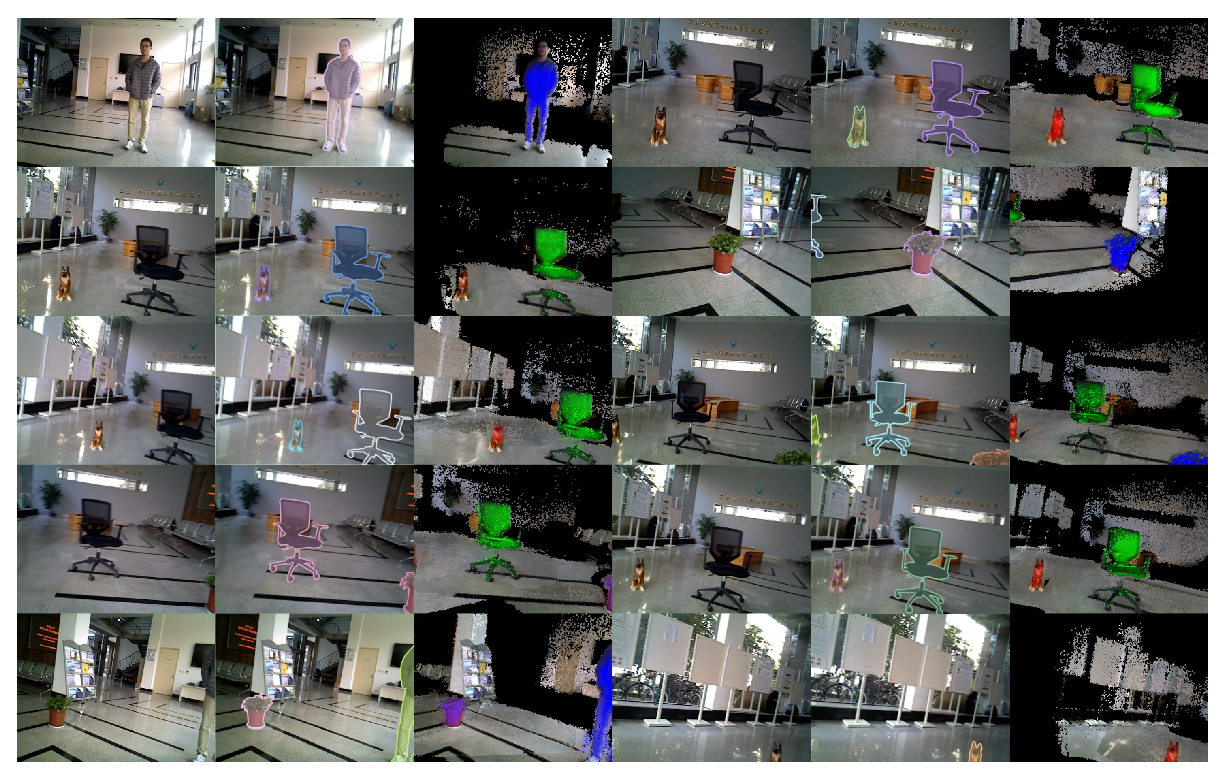
\includegraphics[scale=0.85]{pic/fig2.eps}}
	\put(50,310){Original}
	\put(115,310){Ground Truth}
	\put(200,310){Our Method}
	\put(290,310){Original}
	\put(355,310){Ground Truth}
	\put(440,310){Our Method}
	\end{picture}
	\caption{ {\color{blue}A sketch of our performance on semantic segmentation task. The first and third rows are input images while the second and fourth rows are projection of 3D semantic surfel model of our method.}} 
	\label{fig:fig_sketch}
\end{figure*}  

\section{\textbf{Introduction}}


Understanding the content and the meaning of a perceived scene is a crucial capability for a robot to execute more intelligent behavior.  To solve the core of this problem, the high accuracy of object recognition in 3D scene \cite{Luan2017} and the inclusion of rich semantic information within a dense map is inevitable. As a specific example, suppose a user want his robot to ``fetch the slippers from the shoe rack''. This simple fetching task requires knowledge of both what the target is and what's the shape of it, as well as where it is located. However, even simple as it seems, this fetching task is still challenging for most robots since current SLAM systems are full of geometric information and lack of semantic information. In order to address this challenge, we fuse the high-level features from CNNs with geometric information from SLAM system in order to build a framework which enables a much greater range of functionality and a better understanding of the scene for robots.

Another challenge when adapting CNNs into robots is that although CNNs are widely used in the field of computer vision \cite{Liu2015}, most of the existing CNN-based object detection and semantic segmentation methods are processing of the single 2D frame \cite{long2015fully}, \cite{Zheng2015} which lacks the spatial continuity and temporal consistency of objects. Different pixels of the same object should be continuous in space and the same object appears in the consecutive frames should be close in location. What we need to do is to adjust the CNNs to handle the consecutive frames and preserve the consistency  of space and time. Integrating SLAM system into Convolutional Neural Networks provides a possible solution to preserve time-space consistency. 

The SLAM system beginning as a technique to enable real-time robotic navigation has achieved great success in self-localization, scene reconstruction, and other robotic fields. However, most vision-only SLAM solutions \cite{Whelan15rss}, \cite{Whelan_real-timelarge}, \cite{Zuo2017} which employ simple sparse corner-like features as well as edges, planes, often perform poorly on object detection and reconstruction. For the next level of robot intelligence, maps need to extend beyond geometry — they need to contain semantics \cite{Kundu2014}. The semantics information of objects can open a new perspective for the SLAM system. 

In this paper, we propose a novel framework for object detection and segmentation task based on SLAM system. The foundation of our approach  is built upon a  general 2D object detection Convolutional Neural Networks and a visual SLAM system based on surfel model. All common detection neural networks which output bounding boxes as proposals such as YOLO \cite{Redmon2016}, SSD\cite{Liu2016}, Fast RCNN \cite{Girshick2015}, Faster RCNN \cite{ren2015faster} can be easily transplanted into our framework to be combined with SLAM systems. Objects detected on 2D images are represented as the proposals with its confidence scores.  We use a general object detection framework for each new frame image to obtain the 2D object detection proposals. Then we use SLAM system to predict the estimation proposal for the next frame according to  proposals from previous frame. This process will optimize inter-frame spatial continuity of the object by updating the confidence scores in each frame. The proposals for current frame and estimation results from SLAM are projected into a global 3D surfel model \cite{stuckler2014multi} and update the global target map by pose transformation matrix between new frame and historical  frames, which is obtained by the ICP algorithm for the point clouds registration. Meanwhile, we project the global target map into 2D space and predict new object detection proposals. Therefore, proposals both from CNNs and SLAM are able to fuse together to achieve a better performance on detection task. On the other hand, after filtering the outliers, the fused proposals are used to update the 3D surfel model in SLAM system to label every surfel element semantically. When projecting the filtered surfel model into current 2D perspective, we can obtain the semantic segmentation results.

 


                                                                            

In general, the contribution of this paper can be summarized as follows:
\begin{itemize}
\item By taking advantage of spatial continuity and temporal consistency of objects from SLAM system, we combine knowledge  from single frame ( extracted by Convolution Neural Networks) with knowledge between frames to achieve remarkable progress in accuracy.
\item By combining with SLAM system, we use only one single neural network to accomplish both the detection and the segmentation.
\item We build more grounded and appropriate datasets, evaluate our method on these datasets by comparing with the baseline, which indicates an impressive progress of our method.    
\item We experiment our proposed framework on  benchmarks, compared with state-of-the-art methods on the task of detection and segmentation and prove the effectiveness and the robustness of our approach. 
\end{itemize}

\begin{figure*}[h]
	\centering
	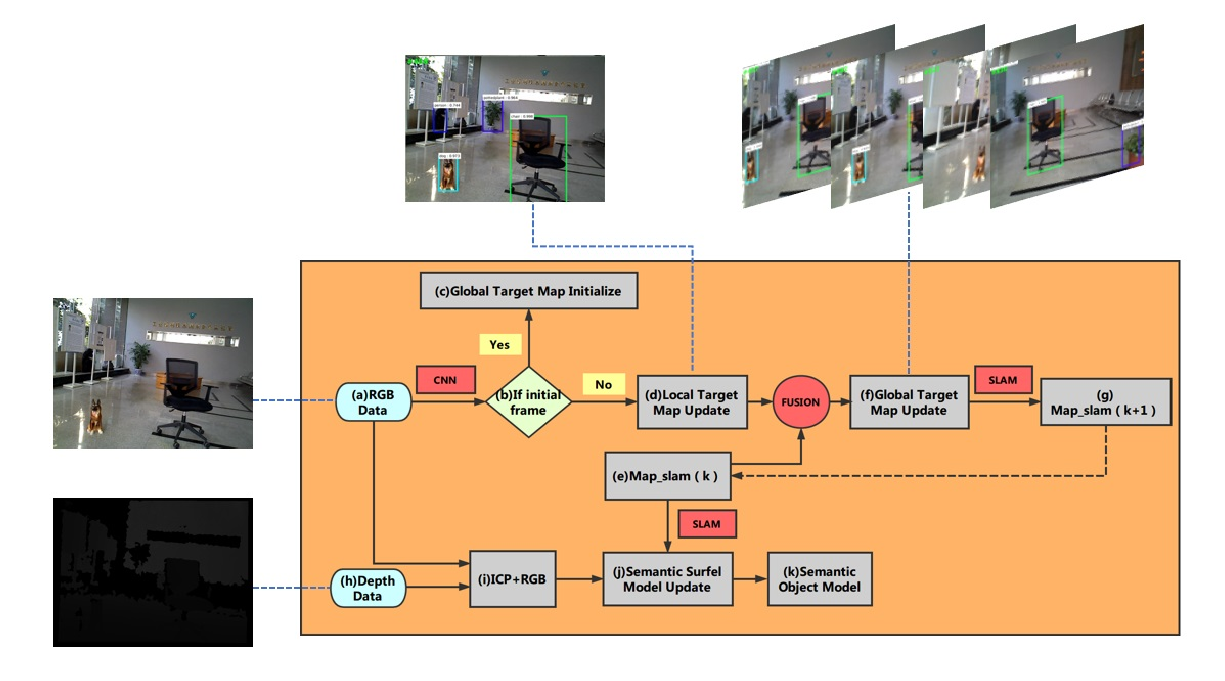
\includegraphics[width=1.0\textwidth]{pic/pipeline.eps}
	\centering
	\caption{{\color{blue}Pipeline of our proposed 3D Object Detection and Segmentation Framework.} (a)The CNNs takes in RGB frame as input (b)First, our algorithm judge if the input frame is initial frame. (c)If the result is yes,  the Global Target Map($Map_{global}$) is initialized{$Map^{0}_{slam}=Map_{global}=boxes$}. (d)If the answer is no,  bounding boxes output from CNNs is used to update the Local Target Map. (e)Target Map from SLAM system ($Map^{k}_{slam}$) at the current moment. (f) Target Map from SLAM system ($Map^{k}_{slam}$)are fused with Local Target Map to update the Global Target Map. (g)Then we use the updated Global Target Map to predict Target Map from SLAM system in the next moment ($Map^{k+1}_{slam}$). (h)The SLAM system also takes depth data as input. (i)ICP+RGB is used for camera attitude estimation. (j)($Map^{k+1}_{slam}$) is used to update the surfel model in the SLAM system. (k)The final semantic map is based on the updated surfel model }
	\label{fig:fig_flowchart}
\end{figure*}



\section{\textbf{Related Work}}

{\color{blue}The field of fusing convolutional neural networks with SLAM system towards building 3D semantic map or obtaining better segmentation results is a hot topic and has yield quite a few works. Among these works, the most related ones are John McCormac et al. \cite{McCormac2017} and Niko S{\"u}nderhauf  et al. \cite{Suenderhauf2017}. John McCormac et al. \cite{McCormac2017} aims to build a dense, semantically annotated 3D map, they combined a specific segmentation neural network by Noh et. al. to provide semantical result and then fuse it with the SLAM system. Unlike them, our framework explore the inherent redundancy among object task and segmentation task, using bounding boxes as intermediate products to segment objects in surfel model and finally build a framework to finish the object detection and segmentation at the same time with one single neural network. Niko S{\"u}nderhauf  et al. \cite{Suenderhauf2017} combined SSD \cite{Liu2016} with SLAM system towards obtain better segmentaion results. Unlike us, They bulid the semantic map based on point cloud and employ depth image to segment objects to construct an adjacency graph.}

Then we discuss related work with respect to the several relevant field that we incorporate within our method, i.e., SLAM, object detection and semantic segmentation.

\textbf{SLAM} SLAM has always been a hot topic in the feild of robotics and there exists a mass of literature on it. Depending on the different  type of input data being processed, SLAM can be divided into either momocular camara-based \cite{Engel14lsd-slam:large-scale}, \cite{Mur-Artal2015}, \cite{Newcombea} or depth camera-based \cite{Keller13real-time3d}, \cite{Whelan_real-timelarge}, \cite{Newcombe}. On the other hand, from the view of methodology, it can be classified as straightforward \cite{Engel}, \cite{Engel14lsd-slam:large-scale}, \cite{Newcombea} or feature-based \cite{Klein2007}, \cite{Klein08improvingthe}, \cite{Mur-Artal2015}. Most feature-based SLAM solutions are mainly based on simple sparse corner-like features such as edges, which tend to perform poorly on semantic level object localization and reconstruction. Under this circumstances, Salas-Moreno et al. \cite{Salas-moreno} come up with a novel approach to create a  semantic annotated SLAM system, SLAM++, which maps indoor scenes at semantically labeled objects level. However, SLAM++ is limited since it only map objects that  exist in a pre-defined database. Additionally, the features it use to match template models are hand-craft.

As for the fusion of  object recognition and SLAM, Sudeep Pillai et al. \cite{Pillai} from MIT propose to combine monocular SLAM with traditional object recognition approach for the first time. They reconstruct the scene in a semi-dense way based on existing monocular SLAM (ORB-SLAM) and import object proposals which are consistent across multiple views into BoVW(Bag-of-Visual-Words) to be classified by traditional well-trained object classifiers. Recently developed deep Convolutional Neural Networks methods \cite{Redmon2016}, \cite{Girshick2015}, \cite{ren2015faster} has significantly outperformed former traditional methods in terms of object recognition accuracy. Therefore, combining SLAM with deep neural networks seem to be a promising solution.

\textbf{Object Detection} 
The last decade has witness the success of HOG \cite{Dalal2005} and SIFT \cite{Lowe2004} due to their achievement in recognition accuracy. These methods are based on block-wise orientation histograms, model the shape of objects via oriented-edge templates, which seems to be less informative when comparing with multi-stage  features extracted by CNNs. In CNN-based state-of-the-art object detection area, there exists two mainstream: models based on region proposals \cite{Girshick2015}, \cite{ren2015faster} and models trained end to end \cite{Redmon2016}, \cite{Liu2016}. End-to-end models like YOLO resize all images into 448 $\times$ 448, utilize features from the whole image to predict bounding boxes and unify separate parts of object detection into one single network. The grid cell proposals is constrained in YOLO, which indicates that the processing time has dropped. But the negative effect is that the detection accuracy for targets, especially small targets, has also declined. Another state-of-the-art techniques in large-scale object detection task is Faster RCNN, which divides the detection process into two procedures: first use a region proposal network to take in input images while outputting rectangular object proposals and then the proposed regions are classified by the Faster RCNN detector network. By sharing computation and using neural networks to propose regions instead of Selective Search, Faster RCNN get a good balance between accuracy and time consumed. However, both models above focus on single frame instead of consecutive frames, thus get a ordinary performance when apply to detection task in consecutive frames.  In this paper, we choose Faster RCNN as our baseline to be compared and it is also the fundamental neural network to be fused into SLAM system.





\textbf{Semantic Segmentation} 
Before the arise of deep learning, approaches such as N-cut \cite{Shi2000} and GrabCut \cite{Rother2004} based on graph partitioning  take the lead in the area of semantic image segmentation. GrabCut proposed by Carsten Rother et.al uses separate Gussian mixture models to model the foreground and background  of a image and seek for the optimal parameters for the models by iteration. But Grubcut need artificial  bounding box or scribbled line as auxiliary information for the sake of achieving a good performance. When it comes to the era of DL (deep learning), Long et al. \cite{long2015fully} first adopt the concept of fully convolutional network(FCN), adapt it on image semantic segmentation and bring us a excellent end-to-end solution. Another cutting-edge innovation is CRF-RNN \cite{Zheng2015}, which brings in the Conditional Random Field to optimize the prediction result after feature extraction. One weakness for DL-based segmentation is that: Both FCN \cite{long2015fully}and CRF-RNN \cite{Zheng2015}need a mass of images and semantic labeled pixels to trained the network. Taking that into consideration, our method costs much less by updating the semantic labels in the 3D map when fusing object proposals from the CNNs. Besides, we save quite a few computation resources and improve the efficiency by using one single neural networks instead of two, because that, as we all known, CNNs are data driven and need plenty of GPU resources to train. 


\section{\textbf{Our Approach}}

In this section, we demonstrate our proposed framework for robot on object detection and segmentation task, where the proposals predicted by CNNs are fused together with the estimation results from the SLAM system. The flow diagram in figure \ref{fig:fig_flowchart} sketches the pipeline of our framework. First of all, the CNNs take in frames to obtain the 2D object detection proposals to form the local target map. Then estimation results from SLAM and the local target map are fused to update the global target map. At the same time, the global target map is projected to 2D to acquire the detection result for current frame. On the other hand, modified RANSAC is adopted to remove the outliers and estimation results from SLAM is sent back to SLAM to update the surfels. In the end, the updated 3D surfel model is projected to 2D to obtain the segmentation result.

The whole framework are mainly connected by three fundamental units: a CNN-based object detection module, a surfel-based SLAM system and a Fusion-Update scheme. The role of CNN module in our framework is to process RGB frames from camera and output a set of candidate bounding boxes with its corresponding probabilities of the target objects. Separately, The SLAM system we used in the framework are ElasticFusion \cite{Whelan15rss}, which provides long-term dense correspondences between frames of  RGB-D video. These correspondences allow the object proposals generated by CNNs from multiple views to be fused into a global consistent sufel-based map. The Fusion-Update scheme uses the correspondences provided by SLAM system to fuse the estimation results from SLAM with the proposals from CNNs and updates the parameters for each target object in both the global target map and the surfel model.


{\color{blue}\subsection{\textbf{CNN Architecture}}

We adopt the classic Faster RCNN by Shaoqing Ren et al. \cite{ren2015faster} as our baseline detection neural network in the framework and the CNN is implemented on caffe \cite{Jia2014}  . As is depicted in figure \ref{fig:CNN architecture}, the original frames are passed through a pre-trained CNN up until an intermediate layer, ending up with a convolutional feature map. We use VGG-16 as a feature extracor in this part. Next, using the features that the CNN computed, the Region Proposal Network (RPN) is adopted to find up to a predefined number of regions (bounding boxes), which may contain objects. Using the features extracted by the CNN and the bounding boxes with relevant objects, Region of Interest (RoI) Pooling is used to extract those features which would correspond to the relevant objects into a new tensor. Finally, comes the R-CNN module, which uses that information to classify the content in the bounding box and adjust the bounding box coordinates. 

The Faster RCNN is pre-trained on Pascal VOC2012. For the training of RPN we adopt standard stochastic gradient descent, with a learning rate of 0.001, momentum of 0.9, and weight decay of 0.0005. The decay policy for learning rate is `step', and the step size is 30000. As for the training of RCNN, the learning rate is 0.001, momentum is 0.9, and weight decay is 0.0005. The decay policy for learning rate is `exp'. We choose a batch size of 64, and train the network for a total of 20k iterations.}

{\color{blue}\subsection{\textbf{Surfel Model}}
	
Surfel model is a method of rendering objects with rich shapes and textures at interactive frame rates and rendering presented in surfel model is based on using simple surface elements (surfels) as rendering primitives \cite{Pfister2000} . Surfels are point samples of a graphics model which is defined as a zero-dimensional n-tuple with shape and shade attributes that locally approximate an object’s surface. We choose surfel model because it is quite appropriate for the modeling of dynamic geometric models which do not need to compute topological information. 

Normally, surfel model is applied on the data representation of medical scanners, real-time particle system rendering and so on. In this work, each surfel in the model stores the following attributes: color information$(R,G,B$), coordinates in 3D space ($x,y,z$), label ($l$), normal vector ($\overrightarrow{n}$)and radius ($r$), initialisation timestamp ($t_{0}$) and last updated timestamp ($t$): 
\begin{equation}
\color{blue}
P_{surfel}=\{x, y, z, (r,g,b), l, r, \overrightarrow{n}\}
\end{equation}
The radius of each surfel represents the local surface area around a given point(which is the optical center of the camera in this work) while minimizing visible holes. 

In the following dynamic modeling process, new surfels are added into the 3D surfel model. Therefore the color, label, location, radius and normal vector are updated in a  weighting fusion way.
}


\subsection{\textbf{Global Target Map}}

We introduce the global target map  in a scene in this subsection. In general, the global target map is the universal set of bounding boxes, which stores the information of each target at each position and one main goal of the fusion scheme is to get the updated  global target map.  As can be seen in the pipeline, after receiving RGB frames by CNN our framework need to judge if the input frame is the initial one. And different answers will result in different procedures. But both procedures involve the target map: If the answer is yes, our algorithm will initialize the global target map, otherwise we will use the proposals from the CNN to form the local target map. Acquiring and updating the global target map is a crucial stage of our framework. 

The global target map, denoted as $Map_{global}$, is defined as the universal set for each object and its corresponding parameters in the whole scene. Correspondently, the local target map $Map_{local}$ is the set of objects and its corresponding parameters for the current frame. Typically, when projecting the global target map into the current camera perspective, we can get the detection result. The output of the CNNs are bounding boxes, denoted as $bdbox_{i}$, and its confidence, denoted as $score_{i}$, with $i$ represents the $ith$ bounding box. We could use four parameters to locate bounding box: $x_{left}$, $y_{top}$, $width$, $height$. 
Then, we can get an example element (denoted as boxI) of the global target map: 
\begin{equation}
boxI=\{x_{leftI},y_{topI},width{I},height{I},score{I}\}
\end{equation} 
As a result, the four endpoints of a bounding box can be described as follows:
\begin{align}
&(x_{left}, y_{top}) =(x_{left}, y_{top}) \\
&(x_{left}, y_{bottom})=(x_{left}, y_{top}+height) \\
&(x_{right}, y_{top})=(x_{left}+width, y_{top}) \\
&(x_{right}, y_{bottom})=(x_{left}+width, y_{top}+height)
\end{align} 
As can be seen from figure \ref{fig:fig_flowchart}, the update of global target map is a dynamic process which involves the local target map($Map_{local}$) derived from CNNs and estimation results from SLAM system($Map_{slam}$). Both of them are fused with each other continuously to update the global target map: Simply speaking, if proposals for a target from CNNs are consistent with estimation results from SLAM, the confidence score for the target will increase, vice versa. The whole update procedures for the global target map are described detailedly in algorithm \ref{alg:update}.


\begin{algorithm}[h]  
	\caption{ Procedures of updating the global target map.}  
	\label{alg:update}  
	\begin{algorithmic}[1]  
		\Require  
		The target bounding boxes  for each frame, denoted as $boxes$; 
		\Ensure  
		The final global map  after fusion and update; :$Map_{global}$;
		\If  {$Initial \  frames$} \\	
		 Initialize the global target map: $Map^{0}_{slam}=Map_{global}=boxes$;  
		\Else 
		\State (1) Get $Map_{local}$ by projecting $Map_{global}$ into current perspective, preserve other targets  beyond the scope of current perspective as: $Map_{tmp}$;
		\State (2) Remove the boxes under the threshold by function $MIX$: $Map_{local}=MIX(boxes,Map_{local})$ ;
		\State (3) Put the updated local target map into the global target; map: $Map_{global}=MIX(Map_{tmp},Map_{local})$;
		\State (4) Fuse the current global target map with the predicted target map from SLAM: $Map_{global}=MIX(Map^{k}_{slam},Map_{gloabl})$;
		\State (5) Get the prediction for the next frame from current global target map: $Map^{k+1}_{slam}=predict(Map_{global})$;
		\EndIf
	\end{algorithmic}  
\end{algorithm} 

The Mix function in algorithm \ref{alg:update} is used to fuse the results from both inputs, which are consist of two subsidiary functions: $reward$ and $punish$. The definition of MIX is shown in algorithm \ref{alg:Mix}. LabelA, labelB are labels of elements  in $Map_{A}$, $Map_{B}$ respectively  and $IOU$  means Intersection over Union:\\
\begin{equation}
IOU(A,B)= (A \cap  B) / (A\cup  B)
\end{equation} 

Function $mix$ and $punish$  are defined as follows:
\begin{equation}
\left.\begin{aligned}
&reward(boxA,boxB)= \{\frac {x_{leftA}+x_{leftB}}{2},\frac {y_{topA}+y_{topB}}{2},\\
&\frac {width_{A}+width_{B}}{2},\frac {height_{A}+height_{B}}{2},\\
&{\color{blue}\frac {(score_{A}+score_{B})\theta_{conf}}{2}\}}
       \end{aligned}
\right\}
\end{equation}
\begin{equation}
\color{blue}
\left.\begin{aligned}
	&punish(boxA,boxB)= decay(boxA\ or\ boxB)= \\
	&\{x_{leftA},y_{topA},width_{A},height_{A},\theta_{punA}score\} \\
	&or \{x_{leftB},y_{topB},width_{B},height_{B},\theta_{punB}score\} 
	\end{aligned} 
\right\}
\end{equation}

$\theta_{conf}$ is a parameter to raise the scores when both sets find the same target. $\theta_{conf}$ is taken to be 1.06  by cross validation and the maximum for the score of a box is 1. Correspondingly, $\theta_{punA}$ and $\theta_{punB}$ are parameters to punish the scores due to the mismatching of two sets. Normally, the appropriate value for $\theta_{pun}$ is 0.94 by cross validation. However, when mixing $Map_{tmp}$ with $Map_{local}$, the value is set as 1 since we need to combine the local target map with new targets to complete the global target map.

\begin{algorithm}[htb]  
	\caption{ Function MIX.}  
	\label{alg:Mix}  
	\begin{algorithmic}[1]  
		\Require 
		$Map_{A},Map_{B}$
		\Ensure  
		$Map_{C}$
		\State Suppose $Map_{C}=MIX(Map_{A},Map_{B})$ 
		\ForAll {$boxA$ in $Map_{A}$}
		\If {IOU(boxA,boxB)$>$threshold and labelA=labelB}
		\State $Map_{C}=reward(boxA,boxB)$
		\Else 
		\State $Map_{C}=punish(boxA,boxB)$
		\EndIf
		\EndFor\\
		\Return 	$Map_{C}$; 
	\end{algorithmic}  
\end{algorithm} 
\subsection{\textbf{SLAM Prediction Map(Map\_slam)}}

In our object detection and segmentation Fusion-Update scheme, there are two kinds of information need to be fused together: proposals from CNNs (in the form of local target map) and predictions from SLAM (in the form of $Map_{slam}$). During the fusion process, we update the global target map and obtain the $Map^{k+1}_{slam}$ by SLAM. Then $Map^{k+1}_{slam}$ is sent back to be fused with the next local target map, as is shown as dotted portion in figure \ref{fig:fig_flowchart}. Since proposals from CNNs are regular bounding boxes with coordinates, we focus on  how to get the predictions for the $(k+1)th$ frame from the $kth$ frame in this subsection.

Suppose the current frame is $k$ and the SLAM systems' prediction of the target map for the next frame is denoted as $Map^{k+1}_{slam}$, we can get the 3D coordinates for a target point of the $kth$ frame in the world coordination by:
\begin{small}
	\color{blue}
	\begin{align}
	z_{k}&=z_{w} \\
	x_{k}&=\frac{(u_{k}-c_{x})z_{k}}{f_{x}} \\
	y_{k}&=\frac{(v_{k}-c_{y})z_{k}}{f_{y}} 
	\end{align}
\end{small}
where $u_{k}, v_{k}$ is the 2D coordinates of the target bounding box's central point in the image coordination. As the depth data obtained from depth image contains holes, to eliminate the instability by adopting data from one single point,  we use the mean depth value of a small patch around the target bounding box's central point to replace the original depth data. 

The coordinate relationship between the $kth$ frame and  the $pth$ frame is defined as:
\begin{small}
	\begin{equation}
	\color{blue}
	\left[\begin{array}{c}
	x_{p}\\
	y_{p}\\
	z_{p}\\
	1
	\end{array}
	\right]
	=inv(tanrsf_{p} / transf_{0})(tanrsf_{k} / transf_{0})
	\left[\begin{array}{c}
	x_{k}\\
	y_{k}\\
	z_{k}\\
	1
	\end{array}
	\right]
	\end{equation}
\end{small}

where $transf_{0}$ is the initial pose matrix while $transf_{p}$ and $transf_{k}$ is the corresponding pose matrix for the $kth$ frame and the $pth$ frame. Then we can project the  $pth$ frame's  3D coordinates into 2D:
\begin{small}
	\begin{align}
	&{\color{blue}u_{p}=\frac{f_{x} x_{p}}{z_{p}}+c_{x}} \\
	&{\color{blue}v_{p}=\frac{f_{y} y_{p}}{z_{p}}+c_{y} }
	\end{align}
\end{small}
By these transformations we can get the predicted bounding box of a target object in the $pth$ frame from the $kth$ frame, as can be shown in figure \ref{fig:chair}. 
\begin{figure}[htb]
	\centering
	\includegraphics[width=0.5\textwidth]{pic/fig4.png}
	\centering
	\caption{Prediction from $kth$ frame to $pth$ frame. Left: Bounding box of the target chair in the $kth$ frame. Right:The predicted bounding box of the target chair in the $pth$ frame.}
	\label{fig:chair}
\end{figure}  

\begin{figure*}[htb]
	\centering
	\includegraphics[width=1\textwidth]{pic/fig3.png}
	\centering
	\caption{{\color{blue}Faster RCNN architecture: Object detection architecture of Shaoqing Ren et al. \cite{ren2015faster} used in our framework.}}
	\label{fig:CNN architecture}
\end{figure*}  


\begin{figure*}[htb]
	\centering
	\includegraphics[width=1\textwidth]{pic/fig5.jpg}
	\centering
	\caption{Examples frbbom self-build datasets.  From Left row to Right row: I, II, III, IV}
	\label{fig:examples}
\end{figure*} 

\subsection{\textbf{3D Surfel Model Update and Semantic Label Fusion}}

Previous segmentation architectures such as SemanticFusion \cite{McCormac2017} mostly use deep models that are tailored to solve one specific task, i.e., semantic segmentation. They do not explore the inherent redundancy among different tasks, which can be formulated by geometry regularities via the nature of 3D scene understanding. Besides, large corpus of labels for pixel are needed to train a traditional deep segmentation neural network in order to preserve high performance with more general scenarios. Nevertheless, Our ObjectFusion framework can finish the segmentation task by processing  the detection results from the  object detection deep neural network in the framework and label the elements in surfel model \cite{stuckler2014multi} from SLAM system, which will eventually reconstruct a 3D semantic surfel model for the scene. The whole update procedures for surfel model is presented in  algorithm \ref{alg:surfel}.

\begin{algorithm}[h]  
	\caption{ Procedures of updating surfel model.}  
	\label{alg:surfel}  
	\begin{algorithmic}[1]  
		\Require  
		surfel model; $Map_{slam}$ 
		\Ensure  
		3D semantic surfel map
		\If  {$Initial frames$} \\	
		Initialize the surfel model
		\Else 
		\State (1) Project $Map_{slam}$ into surfel model to update the parameters(label, probability) of each corresponding surfel elements in the model;
		\State (2) Searching the maximal cluster in these surfel elements;
		\State (3) Label the surfel elements in this maximal cluster as the target object;
		\State (4) Project the surfel model in to 2D and we can get the semantic segmentation result.
		\EndIf
	\end{algorithmic}  
\end{algorithm} 

In consideration of the spatial continuity of objects in a frame, we filter the surfel model based on the spatial location.  More specifically, for each object proposal, we use RANSAC for removing the outliers by sampling. For the clusters on the location of surfel model elements, we search and discard the largest plane, which is mostly likely to be the background. The left largest cluster in the remaining model of this object proposal is what the filtered object proposal. The filtered surfel model preserves the spatial coherence and improves the accuracy of segmentation by segment the bounding box of objects. The estimation error of the camera pose will accumulate over time. Therefore, we calculate the residual loss of the two viewpoints for the new frame and the history frames to determine whether or not to take the local loop closure detection. The local loop closure detection is based on deformation graph \cite{sumner2007embedded} which has been widely used in mesh deformation and non-rigid reconstruction. In addition, We encode raw RGB-D data and the pixel level semantic labels as 5 channels features into binary codes with Random Ferns method \cite{ozuysal2010fast} for the global loop closure detection. The accuracy of the estimation of camera pose can benefit from the local loop closure detection and global semantic loop closure detection.   

Before removing the outliers, we need to update the label and probabilities for each element in surfel model. Let's consider $P(O=l_{i}\mid I_{k})$ denotes the probabilities for target object  from $Map_{slam}$, and former parameters from sufel model, denoted as $P(l_{i}\mid I_{1,...,k-1})$. They are fused together to obtain the updated prediction results:

\begin{equation}
P(l_{i}\mid I_{1,...,k})=\frac{1}{X}P(l_{i}\mid I_{1,...,k-1})P(O=l_{i}\mid I_{k})
\end{equation}
which is applied to all label probabilities per surfel, finally normalizing with constant Z to yield a proper distribution
According to the above equation, the label of surfel element is based on probability which updates every frame. The final label is the one with the maximum probability. If the new-coming frame has the same label with the  history  record, the probability increases and  vice versa:
\begin{equation}
P(\hat{M}^{surfel}_{labeli})=\lambda P(M^{surfel}_{labeli})
\end{equation}
\begin{equation}
\lambda = \lambda [1-(2\times \lvert sgn(label^{p}_{old}-label^{p}_{new} )\rvert-1)]\times \theta_{\lambda}]
\end{equation}
When the current label match the historical one, the output of function $sgn$ is 0 and $\lambda = \lambda\times(1+\theta_{\lambda})$ otherwise $sgn$ would output 1 and  $\lambda =\lambda\times(1-\theta_{\lambda})$.
$\theta_{\lambda}$ is a constant, normally is taken to be 0.96 by cross validation. 

We take advantage of depth data, history record as well as $Map_{slam}$  to update the surfel model's parameters(location, color, label) in SLAM. Since the SLAM prediction map( $Map_{slam}$ ) includes planes such as ground and other objects besides target object, we should remove these disturbed elements in the surfel model to make sure the label for each surfel element is accurate. We adopt RANSAC(Random Sample Consensus) \cite{Fischler1981} to remove the ground. Unlike common RANSAC,  we tend to choose three point ($x_{1},y_{1},z_{1}$), ($x_{2},y_{2},z_{2}$), ($x_{3},y_{3},z_{3}$) around the bounding box as the initial set instead of choosing randomly in the surfel database, which improves the efficiency of finding the background. These three points can establish a plane. By computing the distance between other points and this plane we can count the points near the plane. By update the initial set we can find the plane that have most points near it. That's the target plane which we called outliers to be removed. 

After removing the outliers by RANSAC we still need to filter the surfel model in order to discard disturbed objects. Since each proposal from CNNs contain only one target object, we can accomplish the filtering process by finding the maximal cluster. The searching procedures are presented in algorithm \ref{alg:filter}.

\begin{algorithm}[htbp]  
	\caption{ Searching the maximal cluster in surfel model.}  
	\label{alg:filter}  
	\begin{algorithmic}[1]  
		\State  Using Kd-tree to store Set P;
		\State  Initialize Set C and Set Q as Null Set;
		\For {$p_{i}$ $\in$ P} 
		\State  Add  $p_{i}$  into  Q;
		\EndFor
		\For {$p_{i}$ $\in$ Q} 
		\State Find the neighbourhood of Set $P^k_{i}$ for $p_{i}$;  if d($p_{i}$, $q_{i}$)$<$threshold: $q_{i}$ $\in$ $P^k_{i}$ ; (d($p_{i}$, $q_{i}$) is the Euclidian Distance)
		\EndFor
		\ForAll  {{$q_{i}$ in $P^k_{i}$}}, 
		\State if not processed, add into Q;
		\State After every element in Q is processed, count the number of Q and C, replace C with the bigger one and reset Q as Null Set;
		\EndFor
		\State After every element in P is processed, return C.
	\end{algorithmic}  
\end{algorithm} 

In the end, Our system reconstruct the 3D semantic map based on surfel model and depth camera in an incremental way. By projecting the 3D semantic map to 2D image, we can get the segmentation result. 


\section{\textbf{Experiments}}

In this section, we carry out experimental evaluation to validate the contributions of our proposed approach in terms of detection and semantic segmentation, by means of both qualitative and quantitative comparison against the state-of-the-art methods on four datasets.

Our experiments are carried on desktop PC with an Intel Xeon E5-2620 v3 CPU  at 2.4GHz with 16GB of RAM and a Nvidia Tesla K40C GPU with 12GB of VRAM. As for the implementation of the Convolutional Neural Networks, we choose Faster RCNN as our fundamental detection neural framework and the CNNs are implemented on caffe \cite{Jia2014} and pre-trained on PASCAL VOC2012 \cite{Hoiem}dataset.


\begin{figure*}[htbp]
	\centering
	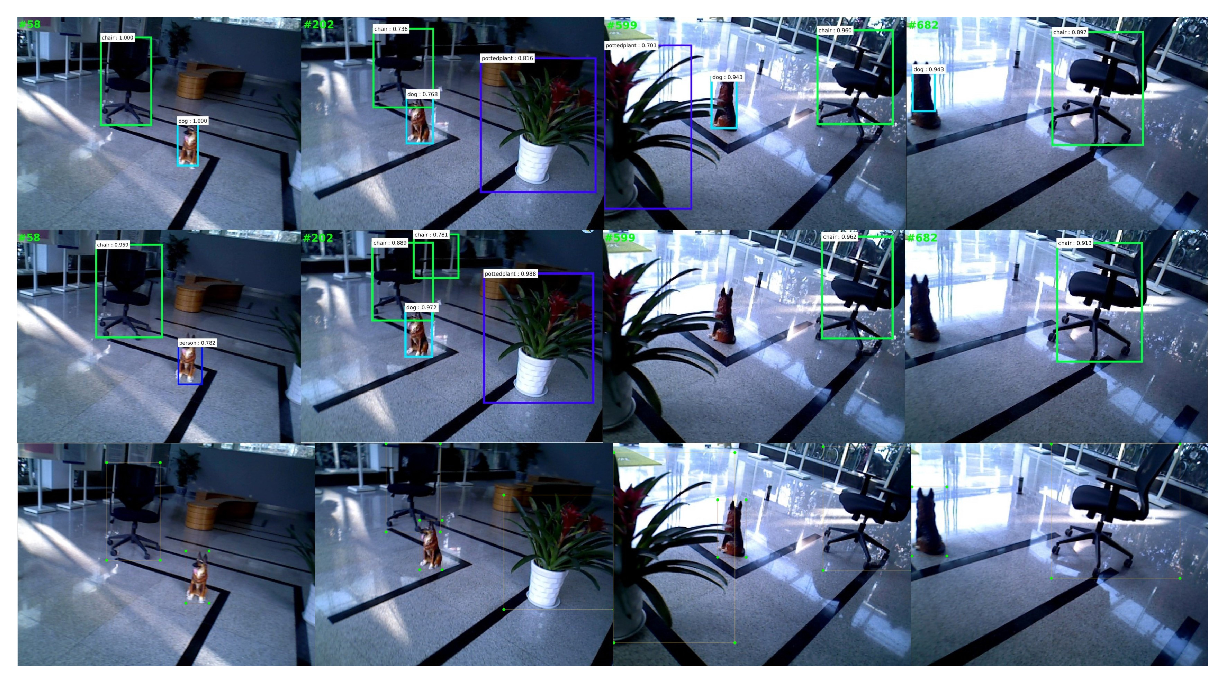
\includegraphics[width=1\textwidth]{pic/fig6.eps}
	\centering
	\caption{ {\color{blue}Detection bounding boxes results in both methods. The first row is the Ground Truth, the second row is Faster RCNN and the third row is our method.}}
	\label{fig:fig_detection}
\end{figure*}

\begin{table*}[htbp]
	\centering
	\normalsize
	\caption{{\color{blue}Comparison with Faster RCNN on Different Data Sets}}
	\label{t1}
	\begin{tabular}{lcccc}
		\hline
		Datasets & Algorithm & {\color{blue}Micro-Precision} &{\color{blue}Micro-Recall} &{\color{blue} Micro-F-measure}\\
		\hline
		\multirow {2}{5cm}{ Dataset I (Single Object)}&2D Faster RCNN baseline&0.6553&\textbf{0.9898}&0.7885\\	
		&Our proposed method&\textbf{0.8694}&0.9025&\textbf{0.8856}\\
		\cline{1-5}
		\multirow {2}{5cm}{ Dataset II (Multiple Objects)}&2D Faster RCNN baseline&0.7632&\textbf{0.8056}&0.7838\\
		&Our proposed method&\textbf{0.9032}&0.7778&\textbf{0.8358}\\	
		\cline{1-5}
		\multirow {2}{5cm}{ Dataset III (Multiple Objects with occlusion)}&2D Faster RCNN baseline&0.8032&\textbf{0.8492}&0.8256\\	
		&Our proposed method&\textbf{0.907}&0.8058&\textbf{0.8534}\\	
		\cline{1-5}
		\multirow {2}{5cm}{ Dataset IV (Multiple Objects with moving obstacles )}&2D Faster RCNN baseline&0.7727&\textbf{0.7391}&0.7555\\	
		&Our proposed method&\textbf{0.9459}&0.7309&\textbf{0.8246}\\
		\hline
	\end{tabular}
\end{table*}

\subsection{\textbf{Dataset}}

Considering most relative existing datasets such as  NYUv2 \cite{Silberman2012}  {\color{blue}do not} provide significant variations in viewpoints for a given scene and the correspondence between depth image and RGB image is not always consistent, we choose to build our own test datasets by collecting RGB-D images using the Xtion live pro depth camera, which aims for a relatively reconstruction of an indoor scene. The trajectory we choose to build the datasets are notably more loopy, both locally and globally. We believe the trajectory in our dataset is more representative of the scanning motion when inspecting a scene. Examples from the four datasets are shown in figure \ref{fig:examples}.

The first dataset (Dataset I) is a single target dataset, collecting in indoor scene with enough light. It consists 1801 successive frames. The second dataset (Dataset II) is multiple targets dataset, which contains multiple objects such as chairs, dogs, pot plants and so on. Dataset II is collected with changing light and composed of 1625 successive frames. Dataset III and IV are more challenging: Dataset III contains multiple objects with occlusion while dataset IV add moving obstacles. We also annotate each image in the four datasets manually. 

\subsection{\textbf{Frame Selection and Convergence {\color{blue}Verification}}}
There is no need to process every frame in actual practice, since the detection results between adjacent frames are analogous. In order to maintain a high processing efficiency, not all frames are processed by the framework, we use reasonable strategy to select target frames in a reasonable way: we design an experiment to evaluate the relationship between accuracy and frames skipped. We evaluate the performance of our CNN framework when performing a prediction on every $2^{n}$ frames, n $\in$ {0,1,..,7}. As is shown in figure \ref{fig:fig_keyframe}, when n$\leq$2, the accuracy almost remain unchanged. By deploying Tesla K40, the average time for processing a image is 0.237s. Therefore, we can improve the efficiency by 4$\times$ when choosing n=2. 

\begin{figure}[htbp]
	\centering
	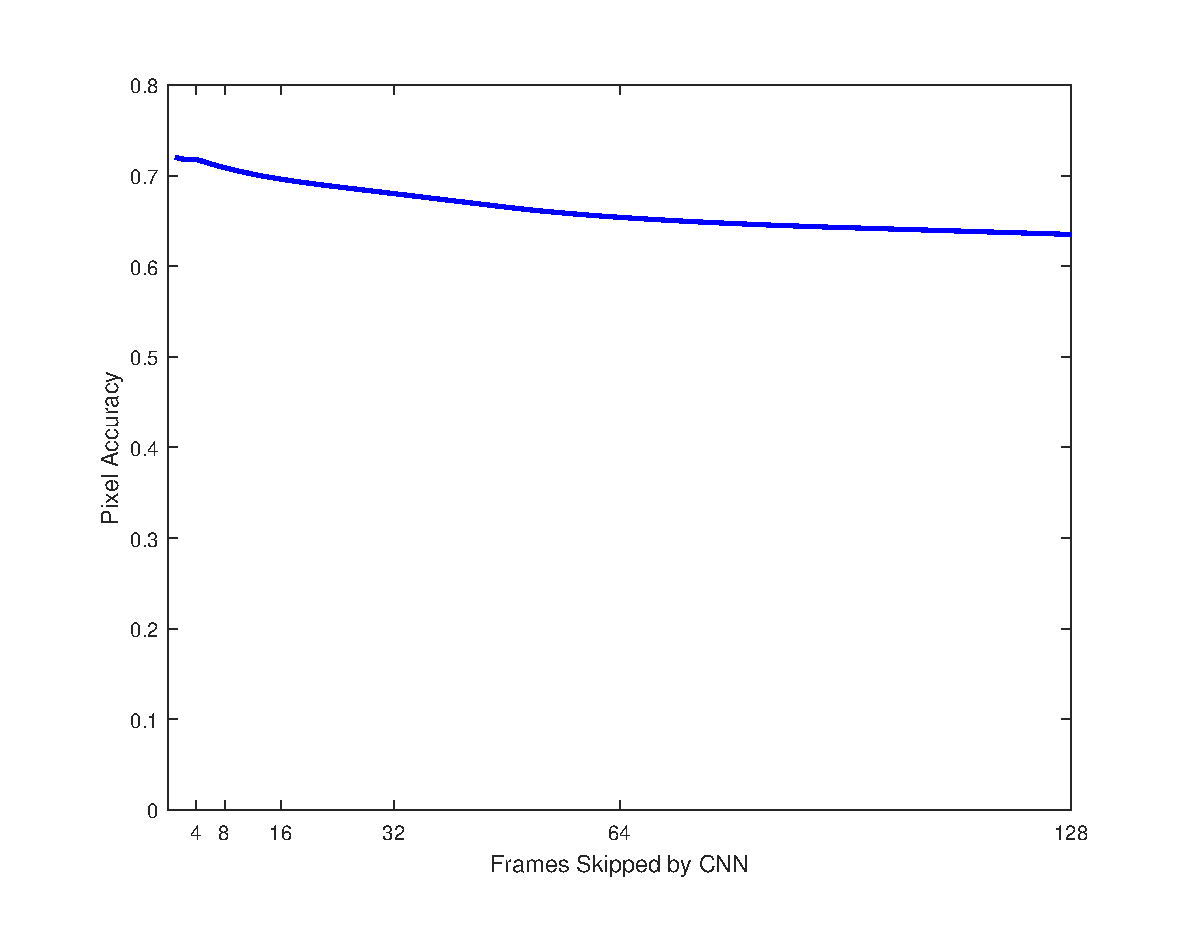
\includegraphics[width=0.5\textwidth]{pic/key_frame.eps}
	\centering
	\caption{The average class accuracy of our RGB-D based method on the single object dataset against the number of frames skipped between fusing semantic predictions.}
	\label{fig:fig_keyframe}
\end{figure}

The SLAM system we used depends on surfel model to label the elements. Each label {\color{blue}can not} generate immediately since the existing surfel database need  evidences from new surfels to update the informations such as location, label, probability and so on. However, the surfels will be updated to the global map only when the confidence score has surpassed the threshold. As a result, the first few frames are not able to label all of the surfels that belong to the object when first recognizing it. Therefore, we need to measure how many frames are necessary before an acceptable semantic surfel model map can be reconstructed. Figure \ref{fig:fig_convergence} is the process of reconstruct a chair in the indoor scene. We can figure out that when it comes to the 10th frame, the object's reconstruction map is on the edge of convergence. Therefore, the first ten frames are removed in the following experiments to guarantee the comparability between our framework and the compared methods.

\begin{figure}[htbp]
	\centering
	\includegraphics[width=0.5\textwidth]{pic/fig10.png}
	\centering
	\caption{Object Reconstruction Map Convergence Vertification Test}
	\label{fig:fig_convergence}
\end{figure} 



\subsection{\textbf{Object Detection Performance}}

Based on the same criterion with Faster RCNN \cite{ren2015faster}, when $IOU$(Intersection over Union) $\ge$ 0.7,  the test result is defined as hit the true value. Under this circumstances, we use the {\color{blue} $precision$}, $recall$ and $F-measure$ as an evaluation criteria for different methods:
\begin{small}
	\begin{align}
	&{\color{blue}precision=\frac{n_{tp}}{n_{tp}+n_{fp}}} \\
	&{\color{blue}recall=\frac{n_{tp}}{n_{tp}+n_{fn}} }\\
	&{\color{blue}F-measure=\frac{2\times precision \times recall}{precision+recall}}
	\end{align}
\end{small}
$n_{tp}$ means the number of predictions that hit the true value, while $n_{fp}$ means the number of predictions that hit the wrong value. $n_{fn}$ represents the number of predictions fail to detect the target. {\color{blue}In order to take into account the possible imbalance among object classes, we compute the $precision$, $recall$ and $F-measure$ in a micro way.}
We evaluate the accuracy of our {\color{blue}ObjectFusion} pipeline against that of achieved by a single frame CNN framework. The quantitative results can be seen in Table \ref{t1}.




\begin{table}[htbp]
	\centering
	\small
	\caption{ {\color{blue}Comparison with FCN,CRF-RNN and Mask RCNN on Dataset I}}
	\label{t2}
	\begin{tabular}{lcccc}
		\hline
		Category& Algorithm& IOU& Pixel Accuracy& Precision \\
		\hline
		\multirow {4}*{Chair}&FCN-voc8s&0.5211&0.6239&0.7923\\
		
		&CRF-RNN&0.5925&0.6373&0.9386\\
		&{\color{blue}Mask RCNN}&{\color{blue}0.5960}&{\color{blue} 0.6451} &{\color{blue} 0.8954}  \\
		
		&SORS(global)&\textbf{0.713}&\textbf{0.726}&\textbf{0.954}\\
		
		&SORS(active)&0.7022&0.724&0.9366\\
		\cline{1-5}
	\end{tabular}
\end{table}

From Table \ref{t1}, we can draw a conclusion that our proposed method remarkably improve the {\color{blue}precision} at the cost of a slight decline of recall rate. The reason why the recall rate drop is that the fused detection system will remove some detected objects that only exist on a single view. Nevertheless, from the result of F-measure,  a more comprehensive evaluation criterion that balance the {\color{blue} $precision$ }and $recall$, we can draw a conclusion that our framework performs steadily better than the baseline(Faster RCNN).   

The qualitative performance is shown in figure \ref{fig:fig_detection}. It can be seen that even for object with part of which exists in the image, our method can successful recognize it because of predictions from the global target map. Besides, evidence from figure \ref{fig:fig_detection} shows that even for object that breaks into the image our system can still detect it smoothly.

\begin{table*}[htb]
	\centering
	\normalsize
	\caption{ {\color{blue}Comparison with FCN, CRF-RNN and Mask RCNN on Dataset II}}
	\label{t3}
	\begin{tabular}{lcccc}
		\hline
		Category& Algorithm& IOU& Pixel Accuracy& Precision \\
		\hline
		\multirow {4}{3cm}{Chair}&FCN-voc8s&0.4596&0.5893&0.4656\\
		
		&CRF-RNN&0.4921&0.5065&0.5219\\ 
		&{\color{blue}Mask RCNN}&{\color{blue}0.5670}&{\color{blue} 0.5971} &{\color{blue} 0.7865}  \\
		
		&SORS(global)&\textbf{0.6396}&\textbf{0.7113}&0.794\\
		
		&SORS(active)&0.5486&0.5789&\textbf{0.8561}\\
		\cline{1-5}
		\multirow {4}{3cm}{Dog}&FCN-voc8s&\textbf{0.49}&\textbf{0.5025}&\textbf{0.8549}\\
		
		&CRF-RNN&0.2827&0.2859&0.2706\\
		&{\color{blue}Mask RCNN}&{\color{blue}0.3213}&{\color{blue} 0.3315} &{\color{blue} 0.4535}  \\
		
		&SORS(global)&0.4727&0.4881&0.7577\\
		
		&SORS(active)&0.4382&0.4513&0.8398\\
		\cline{1-5}
		\multirow {4}{3cm}{Potplant}&FCN-voc8s&0.6012&0.6981&0.8104\\
		
		&CRF-RNN&\textbf{0.656}&0.6781&0.8974\\
		&{\color{blue}Mask RCNN}&{\color{blue}0.5683}&{\color{blue} 0.5778} &{\color{blue} \textbf{0.8976}}  \\
		
		&SORS(global)&0.6545&\textbf{0.7319}&0.8449\\
		
		&SORS(active)&0.6035&0.6994&0.8918\\
		\cline{1-5}
	\end{tabular}
\end{table*}


\begin{table*}[htb]
	\centering
	\normalsize
	\caption{ {\color{blue}Comparison with FCN, CRF-RNN and Mask RCNN on Dataset III}}
	\label{t4}
	\begin{tabular}{lcccc}
		\hline
		Category& Algorithm& IOU& Pixel Accuracy& Precision \\
		\hline
		\multirow {4}{3cm}{Chair}&FCN-voc8s&0.4199&0.5299&0.3887\\
		
		&CRF-RNN&0.4609&0.4788&0.3242\\
		&{\color{blue}Mask RCNN}&{\color{blue}0.416}&{\color{blue} 0.4326} &{\color{blue} 0.3079}  \\
		
		&SORS(global)&\textbf{0.5159}&\textbf{0.5534}&0.9015\\
		
		&SORS(active)&0.4267&0.4465&\textbf{0.9347}\\
		\cline{1-5}
		\multirow {4}{3cm}{Dog}&FCN-voc8s&\textbf{0.4306}&0.4301&0.8545\\
		
		&CRF-RNN&0.3675&0.3715&0.2675\\
		&{\color{blue}Mask RCNN}&{\color{blue}0.3957}&{\color{blue} 0.4012} &{\color{blue} 0.2965}  \\
		&SORS(global)&0.4087&\textbf{0.4768}&0.8001\\
		
		&SORS(active)&0.3635&0.3871&\textbf{0.8683}\\
		\cline{1-5}
		\multirow {4}{3cm}{Potplant}&FCN-voc8s&0.6545&0.7854&0.7009\\
		
		&CRF-RNN&0.612&0.7134&0.6989\\
		&{\color{blue}Mask RCNN}&{\color{blue}\textbf{0.6722}}&{\color{blue} 0.7854} &{\color{blue} 0.7422}  \\
		
		&SORS(global)&0.6669&\textbf{0.7904}&0.9303\\
		
		&SORS(active)&0.6166&0.7499&\textbf{0.9385}\\
		\cline{1-5}
	\end{tabular}
\end{table*}





\subsection{\textbf{Object Semantic Segmentation Evaluation}}

We adopt the classic evaluation criteria in the semantic segmentation field to evaluate our framework : $pixel\ accuracy $, $precision$, $IOU$, $mean\ accurary$, $mean\ IOU$ and $mean\ precision$. $IOU$ in this section is based on the number of the pixels instead of bounding boxes in the previous section. 
\begin{small}
	\begin{align}
	&pixel\ accuracy=\frac{\sum_{i}n_{ii}}{\sum_{i}t_{i}} \\
	&mean\ accuracy=\frac{1}{n_{cl}}\frac{\sum_{i}n_{ii}}{\sum_{i}t_{i}} \\ 
	&IOU=\sum_{i}\frac{n_{ii}}{t_{i}+\sum_{j}n_{ji}-n_{ii}}\\
	&mean\ IOU=\frac{1}{n_{cl}}\sum_{i}\frac{n_{ii}}{t_{i}+\sum_{j}n_{ji}-n_{ii}}\\
	&precision=\frac{\sum_{i}n_{ii}}{\sum_{j}n_{ji}} \\
	&mean\ precision=\frac{1}{n_{cl}}\frac{\sum_{i}n_{ii}}{\sum_{j}n_{ji}} 
	\end{align}
\end{small}

$n_{ij}$ is the number of pixels which classified as $j$ while the true value is $i$. $n_{cl}$ is the total number of all classes. $t_{i}=\sum_{j}n_{ij}$ is the number of pixels that belongs to class $i$.

In this section, our approach, denoted as SORS(SLAM-based Object Recognition and Segmentation), is compared with two existing  state-of-the-art 2D semantic segmentation methods: CRF-RNN \cite{Zheng2015}and FCN \cite{long2015fully}. In the architecture of ElasticFusion \cite{Whelan15rss}, the system separate the scene into active area and inactive area according to the interval between current frame and other frames. We adopt the conception of active areas to update the surfel model. In the quantitative experiments, we perform our algorithm  with two separate strategies:  ``global'' and ``active''. ``Global" means updating the global surfel-based 3D map based on each frame and project the results to 2D planes while ``active" only reconstruct the 3D map for current active areas and project the results to 2D images. Obviously, the ``global'' strategy concerns the whole scene while the ``local" one focus more on adjacent areas. Comparisons on all four datasets can be seen in Table \ref{t2}- Table \ref{t5}.



 \begin{table*}[htbp]
	\centering
	\normalsize
	\caption{ {\color{blue}Comparison with FCN, CRF-RNN and Mask RCNN on Dataset IV}}
	\label{t5}
	\begin{tabular}{lcccc}
		\hline
		Category& Algorithm& IOU& Pixel Accuracy& Precision \\
		\hline
		\multirow {4}{3cm}{Chair}&FCN-voc8s&0.3994&0.452&0.8317\\
		
		&CRF-RNN&0.327&0.3452&0.6331\\
		&{\color{blue}Mask RCNN}&{\color{blue}0.3557}&{\color{blue}0.3817} &{\color{blue} 0.7112}  \\
		&SORS(global)&0.4591&0.4727&0.7597\\
		
		&SORS(active)&\textbf{0.469}&\textbf{0.4776}&\textbf{0.835}\\
		\cline{1-5}
		\multirow {4}{3cm}{Dog}&FCN-voc8s&0.2845&0.3048&\textbf{0.8236}\\
		
		&CRF-RNN&0.154&0.165&0.6147\\
		&{\color{blue}Mask RCNN}&{\color{blue}0.2301}&{\color{blue} 0.2564} &{\color{blue} 0.7074}  \\
		&SORS(global)&\textbf{0.2993}&\textbf{0.3064}&0.7855\\
		
		&SORS(active)&0.2652&0.2739&0.7521\\
		\cline{1-5}
		\multirow {4}{3cm}{Potplant}&FCN-voc8s&0.3747&0.4937&0.5441\\
		
		&CRF-RNN&0.3381&0.3866&0.5387\\
		&{\color{blue}Mask RCNN}&{\color{blue}0.3167}&{\color{blue} 0.4114} &{\color{blue} 0.6002}  \\
		&SORS(global)&\textbf{0.4453}&\textbf{0.4991}&\textbf{0.7965}\\
		
		&SORS(active)&0.3841&0.412&0.7758\\
		\cline{1-5}
		\multirow {4}{3cm}{Person}&FCN-voc8s&0.8048&0.8782&0.7383\\
		
		&CRF-RNN&0.8066&0.8593&0.3553\\
		&{\color{blue}Mask RCNN}&{\color{blue}0.8306}&{\color{blue}\textbf{0.8856}} &{\color{blue} 0.8452}  \\
		
		&SORS(global)&\textbf{0.8338}&0.8848&0.8561\\
		
		&SORS(active)&0.8042&0.8596&\textbf{0.8666}\\
		\cline{1-5}
	\end{tabular}	
\end{table*} 





\begin{figure*}[htbp]
	\begin{picture}(500,220)
	\put(70,0){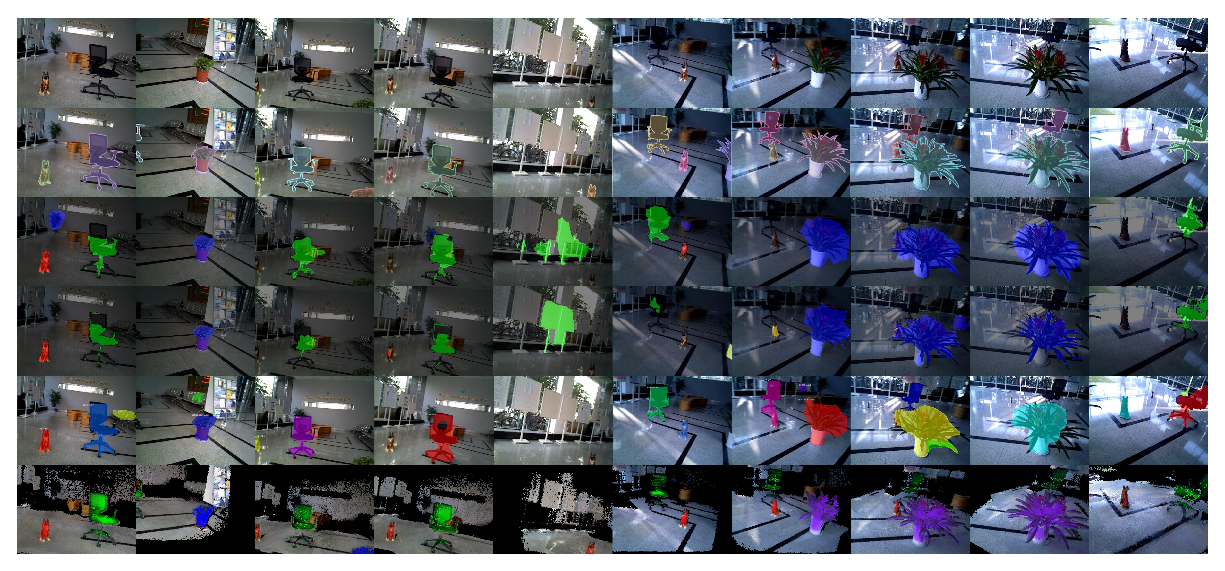
\includegraphics[scale=0.8]{pic/fig9.eps}}
	\put(0,180){Original}
	\put(0,145){Ground Truth}
	\put(0,115){FCN-VOC8s}
	\put(0,80){CRF-RNN}
	\put(0,45){MASK RCNN}
	\put(0,10){Our SORS}
	\end{picture}
	\caption{{\color{blue}Comparation with FCN, CRF-RNN and Mask RCNN on segmentation task}}	
	\label{fig:fig_segmentation}
\end{figure*}   


 \begin{table*}[htbp]
	\centering
	\normalsize
	\caption{ Mean Performance on Different Datasets }
	\label{t6}
	\begin{tabular}{lcccc}
		\hline
		Category& Algorithm& Mean IOU& Mean Pixel Accuracy& Mean Precision \\
		\hline
		\multirow {4}{3cm}{Dataset I}&FCN-voc8s&0.5211&0.6239&0.7923\\
		
		&CRF-RNN&0.5925&0.6373&0.9386\\
		&{\color{blue}Mask RCNN}&{\color{blue}0.5960}&{\color{blue} 0.6451} &{\color{blue} 0.8954}  \\
		
		&SORS(global)&\textbf{0.713}&\textbf{0.726}&\textbf{0.954}\\
		
		&SORS(active)&0.7022&0.724&0.9366\\
		\cline{1-5}
		\multirow {4}{3cm}{Dataset II}&FCN-voc8s&0.5169&0.5966&0.7103\\
		
		&CRF-RNN&0.4769&0.4899&0.5633\\
		&{\color{blue}Mask RCNN}&{\color{blue}0.4855}&{\color{blue} 0.5021} &{\color{blue} 0.7125}  \\
		
		&SORS(global)&\textbf{0.5889}&\textbf{0.6438}&0.7989\\
		
		&SORS(active)&0.5301&0.5765&\textbf{0.8626}\\
		\cline{1-5}
		\multirow {4}{3cm}{Dataset III}&FCN-voc8s&0.5775&0.6559&0.6708\\
		
		&CRF-RNN&0.5618&0.6058&0.4115\\
		&{\color{blue}Mask RCNN}&{\color{blue}0.4946}&{\color{blue} 0.5397} &{\color{blue} 0.4489}  \\
		
		&SORS(global)&\textbf{0.6063}&\textbf{0.6764}&0.872\\
		
		&SORS(active)&0.5528&0.6106&\textbf{0.902}\\
		\cline{1-5}
		\multirow {4}{3cm}{Dataset VI}&FCN-voc8s&0.3529&0.4168&0.7361\\
		
		&CRF-RNN&0.273&0.2989&0.5955\\
		&{\color{blue}Mask RCNN}&{\color{blue}0.3433}&{\color{blue} 0.3938} &{\color{blue} 0.716}  \\
		
		&SORS(global)&\textbf{0.4012}&\textbf{0.4261}&0.7806\\
		
		&SORS(active)&0.3728&0.3878&\textbf{0.7873}\\
		\cline{1-5}
	\end{tabular}	
\end{table*}

\textbf{Discussion}  
Table \ref{t2} - Table \ref{t5} show that the semantic segmentation become increasingly challenging as the scene tends to be more complicated. Nevertheless, we can see that our method prevails in all four datasets, especially in the results of pixel accuracy and IOU, which are more important because the precision only take samples that are recognized as positive into account.

One detail we can see from Table \ref{t2} - Table \ref{t5} is that our SORS make a big progress in the segmentation of chair while only improved within limits when it comes to dog. Apparently, chairs are more difficult to be recognized and segmented due to the wheels and discrete shape. But our method could handle these details quite well and get a better performance by combining with SLAM. In addition, our SORS algorithm is able to segment more detailedly such as the branches and leaves of pot plant, human arms and legs, etc. Qualitative comparisons are presented in figure \ref{fig:fig_segmentation} .

Another phenomenon from Table \ref{t2} - Table \ref{t5} is that sometimes the performance of ``active" is better than ``global", especially in Dataset IV. That's because the global map is designed to fuse with each frame. If our CNNs framework fail to detect target in several successive frames, the global map will  lower the probability for certain label, which will cause the ineffectiveness of semantic segmentation. However, Average performance in Table \ref{t6} proves that the global SORS algorithm is still more robust and could be a more promising choice.


{\color{blue}\subsection{\textbf{Run-time Performance}}

To evaluate the run-time performance of our framework we perform experiments on a sample of random 20 sequences from the test set. Each sequence last for 5 seconds. The experiments were performed on an Intel® Xeon(R) CPU E5-2620 v3 @ 2.40GHz × 16 CPU and an Nvidia Tesla K40C GPU. It requires 45.6ms on average to process one frame and update the map in the SLAM system. Besides, it need an additional 1.5ms on average to update the surfel model for each chosen frame. As is illustrated above, the other deployments in the framework do not need to be applied for each frame. The average time for a forward pass of our CNN and the update of our global target map on one frame is 121.7ms. And our standard scheme performs this every 4 frames.}



\section{\textbf{Conclusion}}

We have shown that  the integration of SLAM with 2D proposals via a deep neural network is a effective direction to solve the problems of object detection and semantic segmentation. We perform experiments on  single object, multiple objects, occlusion, illumination changes, exist moving obstacle environments with the Asus Xtion Pro RGB-D sensor and show that our model obviously improves the robustness for object detection problem in the rich variety of environments. For the semantic segmentation task, our method is compared to previous 2D methods such as FCN-8s \cite{long2015fully}, CRF-RNN \cite{Zheng2015} and Mask RCNN \cite{He2017}with all of the models trained on Pascal VOC 2012 dataset \cite{Everingham15}. The results demonstrate that our model can obtain a high-quality object semantic segmentation performance. Evaluations reveal our framework is capable of incrementally reconstructing the semantic labeled scene as well as fusing proposals from CNNs, which is a new perspective towards scene understanding and semantic segmentation with RGB-D camera.

A future research schedule going further into exploit more efficient CNN architectures, combining high-level representations from CNNs and low-level representations such as edges, corners from SLAM to reconstruct a more accurate and detailed 3D semantic map.
% For peer review papers, you can put extra information on the cover
% page as needed:
% \ifCLASSOPTIONpeerreview
% \begin{center} \bfseries EDICS Category: 3-BBND \end{center}
% \fi
%
% For peerreview papers, this IEEEtran command inserts a page break and
% creates the second title. It will be ignored for other modes.
\IEEEpeerreviewmaketitle



%\section{Introduction}
%% no \IEEEPARstart
%This demo file is intended to serve as a ``starter file''
%for IEEE conference papers produced under \LaTeX\ using
%IEEEtran.cls version 1.8b and later.
%% You must have at least 2 lines in the paragraph with the drop letter
%% (should never be an issue)
%I wish you the best of success.
%
%\hfill mds
%
%\hfill August 26, 2015
%
%\subsection{Subsection Heading Here}
%Subsection text here.
%
%
%\subsubsection{Subsubsection Heading Here}
%Subsubsection text here.
%
%
%% An example of a floating figure using the graphicx package.
%% Note that \label must occur AFTER (or within) \caption.
%% For figures, \caption should occur after the \includegraphics.
%% Note that IEEEtran v1.7 and later has special internal code that
%% is designed to preserve the operation of \label within \caption
%% even when the captionsoff option is in effect. However, because
%% of issues like this, it may be the safest practice to put all your
%% \label just after \caption rather than within \caption{}.
%%
%% Reminder: the "draftcls" or "draftclsnofoot", not "draft", class
%% option should be used if it is desired that the figures are to be
%% displayed while in draft mode.
%%
%%\begin{figure}[!t]
%%\centering
%%\includegraphics[width=2.5in]{myfigure}
%% where an .eps filename suffix will be assumed under latex,
%% and a .pdf suffix will be assumed for pdflatex; or what has been declared
%% via \DeclareGraphicsExtensions.
%%\caption{Simulation results for the network.}
%%\label{fig_sim}
%%\end{figure}
%
%% Note that the IEEE typically puts floats only at the top, even when this
%% results in a large percentage of a column being occupied by floats.
%
%
%% An example of a double column floating figure using two subfigures.
%% (The subfiguresty package must be loaded for this to work.)
%% The subfigure \label commands are set within each subfloat command,
%% and the \label for the overall figure must come after \caption.
%% \hfil is used as a separator to get equal spacing.
%% Watch out that the combined width of all the subfigures on a
%% line do not exceed the text width or a line break will occur.
%%
%%\begin{figure*}[!t]
%%\centering
%%\subfloat[Case I]{\includegraphics[width=2.5in]{box}%
%%\label{fig_first_case}}
%%\hfil
%%\subfloat[Case II]{\includegraphics[width=2.5in]{box}%
%%\label{fig_second_case}}
%%\caption{Simulation results for the network.}
%%\label{fig_sim}
%%\end{figure*}
%%
%% Note that often IEEE papers with subfigures do not employ subfigure
%% captions (using the optional argument to \subfloat[]), but instead will
%% reference/describe all of them (a), (b), etc., within the main caption.
%% Be aware that for subfiguresty to generate the (a), (b), etc., subfigure
%% labels, the optional argument to \subfloat must be present. If a
%% subcaption is not desired, just leave its contents blank,
%% e.g., \subfloat[].
%
%
%% An example of a floating table. Note that, for IEEE style tables, the
%% \caption command should come BEFORE the table and, given that table
%% captions serve much like titles, are usually capitalized except for words
%% such as a, an, and, as, at, but, by, for, in, nor, of, on, or, the, to
%% and up, which are usually not capitalized unless they are the first or
%% last word of the caption. Table text will default to \footnotesize as
%% the IEEE normally uses this smaller font for tables.
%% The \label must come after \caption as always.
%%
%%\begin{table}[!t]
%%% increase table row spacing, adjust to taste
%%\renewcommand{\arraystretch}{1.3}
%% if using array.sty, it might be a good idea to tweak the value of
%% \extrarowheight as needed to properly center the text within the cells
%%\caption{An Example of a Table}
%%\label{table_example}
%%\centering
%%% Some packages, such as MDW tools, offer better commands for making tables
%%% than the plain LaTeX2e tabular which is used here.
%%\begin{tabular}{|c||c|}
%%\hline
%%One & Two\\
%%\hline
%%Three & Four\\
%%\hline
%%\end{tabular}
%%\end{table}
%
%
%% Note that the IEEE does not put floats in the very first column
%% - or typically anywhere on the first page for that matter. Also,
%% in-text middle ("here") positioning is typically not used, but it
%% is allowed and encouraged for Computer Society conferences (but
%% not Computer Society journals). Most IEEE journals/conferences use
%% top floats exclusively.
%% Note that, LaTeX2e, unlike IEEE journals/conferences, places
%% footnotes above bottom floats. This can be corrected via the
%% \fnbelowfloat command of the stfloats package.
%
%
%
%
%\section{Conclusion}
%The conclusion goes here.
%
%
%
%
%% conference papers do not normally have an appendix
%
%
%% use section* for acknowledgment
%\section*{Acknowledgment}
%
%
%The authors would like to thank...





% trigger a \newpage just before the given reference
% number - used to balance the columns on the last page
% adjust value as needed - may need to be readjusted if
% the document is modified later
%\IEEEtriggeratref{8}
% The "triggered" command can be changed if desired:
%\IEEEtriggercmd{\enlargethispage{-5in}}

% references section

% can use a bibliography generated by BibTeX as a .bbl file
% BibTeX documentation can be easily obtained at:
% http://mirror.ctan.org/biblio/bibtex/contrib/doc/
% The IEEEtran BibTeX style support page is at:
% http://www.michaelshell.org/tex/ieeetran/bibtex/
%\bibliographystyle{IEEEtran}
% argument is your BibTeX string definitions and bibliography database(s)
%\bibliography{IEEEabrv,../bib/paper}
%
% <OR> manually copy in the resultant .bbl file
% set second argument of \begin to the number of references
% (used to reserve space for the reference number labels box)
%\begin{thebibliography}{1}

%\bibitem{IEEEhowto:kopka}
%H.~Kopka and P.~W. Daly, \emph{A Guide to \LaTeX}, 3rd~ed.\hskip 1em plus
%  0.5em minus 0.4em\relax Harlow, England: Addison-Wesley, 1999.

% \end{thebibliography}

\bibliographystyle{plain}
\bibliography{ref}
% that's all folks
\end{document}


